\section*{Abstract}

Demanding work can leave a useful executable asset, but a useful asset is not automatically a scarce or financeable advantage. We implemented and tested a connected scientific-software service: solve sparse grounded networks, recover grouped coefficients from partial observations, and optimize a finite-scenario resource allocation. A source-frozen comparison covered 12 engineering chains, three stages per chain and four methods. All 144 arm-stage evaluations passed independent numerical acceptance. An independent agent's reduced-space design method improved the original recipient's solver time by 9.87 and 129.91 times on two separate fresh cases; the reverse acquisition produced no benefit. Competent independent reconstruction was successful and fastest across the complete primary cohort. A searchable registry and a validated skills graph delivered the same accepted work; no incremental graph advantage was demonstrated. A separately frozen finite-cash market model evaluates complete-category cost scenarios, copying, contribution and reinvestment. Demand and monetary inputs remain assumptions, actual customer receipts are zero, and actual all-in research costs are unknown. The evidence supports selective software retention and a recipient-specific execution improvement. It does not establish a durable scarce-capability advantage or realized self-financing growth.

\section{What the work produced}

The delivered asset is an executable scientific workflow, not a transcript: a sparse forward solver, a bounded inverse-calibration method with independently checked predictions, and a robust design method with a numerical optimality certificate. The final design consumes the receiving method's own accepted inverse parameters. Hidden true coefficients never replace a failed upstream result.

The most useful contribution arose during independent construction. Agent A found that repeatedly factorizing the full network inside design optimization was avoidable. Its implementation reduced the design update to the selected edge subspace, using a Woodbury update, analytic sensitivities and constrained optimization. Root retained this contribution as design version 2 before generating primary evaluation inputs. Design version 1 remains preserved as superseded evidence. These are implementations of public mathematical methods; no new theorem or exclusive algorithm is claimed.

\subsection{A visible transfer, including the unsuccessful direction}

The acquisition panel was declared separately and used two new chains with 625 and 2,500 nodes. All twelve stage-method outcomes passed the same independent verifier. The table reports the design solver call only; process startup, native packaging, acquisition and independent verification are excluded from these timings.

\begin{center}
\begin{tabular}{lrrr}
\toprule
Fresh case & Original recipient & Contributed method & Time ratio\\
 & seconds & seconds & original/contributed\\
\midrule
625 nodes & 0.164216 & 0.016639 & 9.87\\
2,500 nodes & 29.279230 & 0.225381 & 129.91\\
\bottomrule
\end{tabular}
\end{center}

\begin{figure}[htbp]
\centering
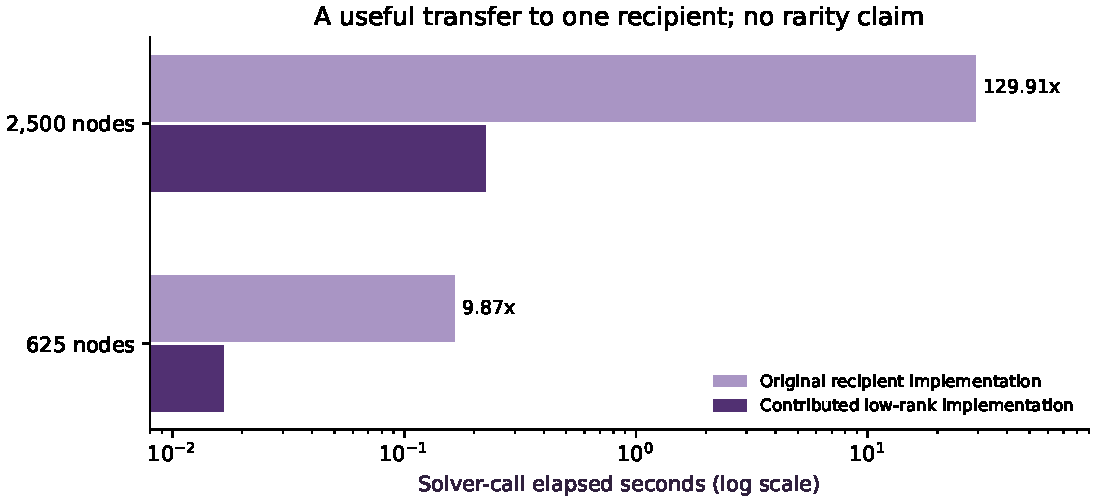
\includegraphics[width=0.94\linewidth]{figures/transfer.pdf}
\caption{An observed implementation advantage for the original recipient. Both methods satisfy the declared numerical contract. This two-case, solver-only comparison does not identify complete monetary acquisition value or a general speedup distribution.}
\end{figure}

The receiving independent agent already possessed the faster method. Importing root's initial capabilities added no accepted task and did not improve its timing. Root's acquisition of the independent contribution is therefore the useful direction. It improves a specific recipient's retained implementation; it does not prove that the independent comparator population lacked the underlying capability. Root's reverse-direction integration time and actual model bills were not separately measured, so a complete observed monetary break-even cannot be computed.

\subsection{Fresh production comparison}

The primary protocol froze all methods and acceptance before input generation. Three fixed seeds at each of four sizes produced 12 independent chains. The four arms were evaluated in a cyclic order, and all 48 inverse outcomes were sealed before downstream design templates were released. No primary repair, favorable substitution or efficacy rerun was used.

\begin{center}
\small
\begin{tabular}{p{0.41\linewidth}rrrr}
\toprule
Arm & Accepted & Complete & CPU & Elapsed\\
 & stages & chains & seconds & seconds\\
\midrule
A: independent retained reconstruction & 36/36 & 12/12 & 99.785 & 98.682\\
B: validated searchable registry & 36/36 & 12/12 & 112.469 & 110.853\\
C: validated skills graph & 36/36 & 12/12 & 114.748 & 113.070\\
D: strong conventional implementation & 36/36 & 12/12 & 182.854 & 181.729\\
\bottomrule
\end{tabular}
\end{center}

These totals include discovery or selection within the invocation, execution, independent numerical checking and the native record boundary. They exclude one-time research construction and catalogue admission, which are recorded separately. All planned rows executed, all complete acceptance budgets were respected, and no additional accepted job was attributable to sharing or graph structure. The 144 evaluations are repeated comparisons of 36 stages in \emph{12 chains}; they are not 144 independent customers or agents.

\begin{figure}[htbp]
\centering
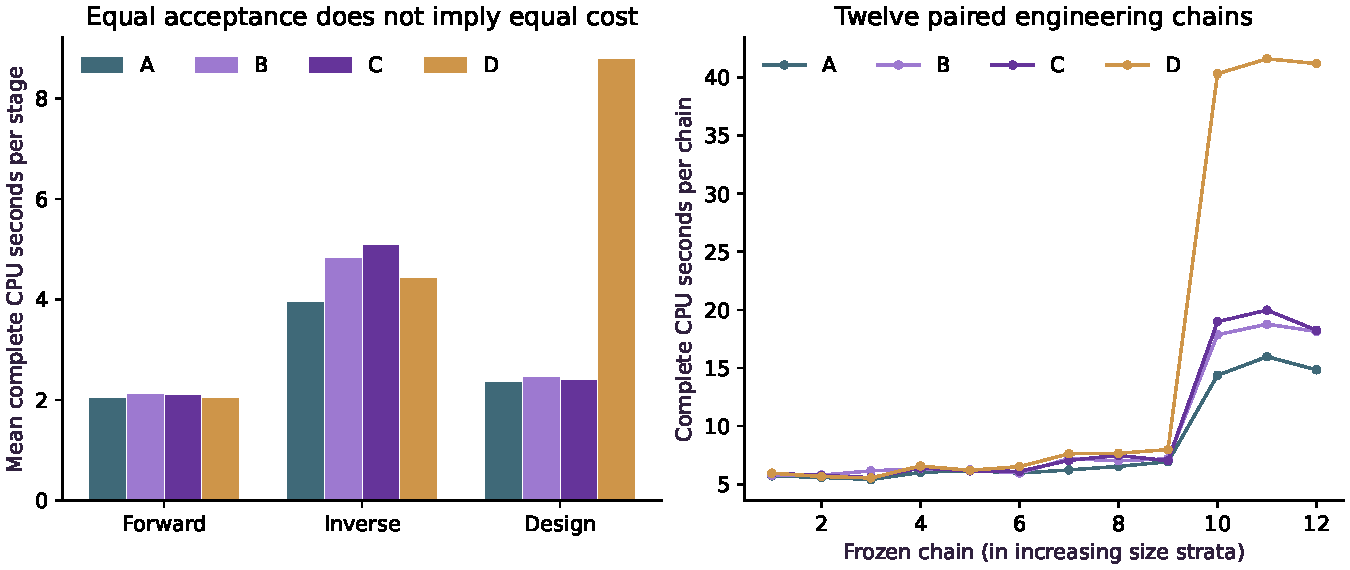
\includegraphics[width=\linewidth]{figures/primary.pdf}
\caption{Complete invocation costs in the frozen primary cohort. Registry and graph use exactly the same selected executable capabilities and evidence. Independent reconstruction remains a strong feasible alternative, including on the largest jobs.}
\end{figure}

The mean paired chain CPU difference was $+1.057$ seconds for B minus A, with a descriptive 95\% chain-bootstrap interval of $[0.403,1.817]$. For C minus B it was $+0.190$ seconds, interval $[-0.066,0.489]$. Positive values consume more CPU. B minus D was $-5.865$ seconds, interval $[-11.569,-0.352]$, primarily reflecting the more efficient design implementation. The intervals resample these twelve chains; they are not population-wide causal estimates, field reliability bounds or evidence about a distribution of foundation models.

\subsection{Success levels and their evidence boundaries}

\begin{center}
\small
\begin{tabular}{p{0.10\linewidth}p{0.25\linewidth}p{0.55\linewidth}}
\toprule
Level & Finding & Supported interpretation\\
\midrule
1 & Demonstrated in scope & Reusable executable numerical capabilities satisfy fresh synthetic engineering requirements. Actual customer demand is unobserved.\\[4pt]
2 & Qualified execution benefit & A contributed implementation improves another recipient's fresh solver performance. No additional feasible job, unsupported baseline capability or complete monetary acquisition benefit is established.\\[4pt]
3 & Not established empirically & Actual complete costs and recurring demand are unidentified. Conditional full-category scenarios are reported separately below.\\[4pt]
4 & Not demonstrated & Graph and competent registry have equal acceptance; graph CPU advantage is not shown, and extra graph authoring cost is unknown.\\[4pt]
5 & Not demonstrated & Actual customer collections are zero; no later-investment bundle qualifies in either sharing arm's 2,304 modeled worlds.\\[4pt]
6 & Not demonstrated & No difficulty-adjusted sequence of independently measured development and validation efficiencies was executed.\\
\bottomrule
\end{tabular}
\end{center}

The result is deliberately narrower than the requested commercial demonstration sentence. This recipient already could complete the work; it completed fresh design work faster after acquisition. The study cannot truthfully replace that finding with ``could not economically perform'' when actual acquisition costs, demand and best-alternative commercial prices are unknown.

\section{Financial results: useful instances, no financed succession}

The market campaign completed all 144 condition/cost cells and 2,304 paired worlds, producing 9,216 primary enterprise histories and 46 additional same-world financing controls. It took 61.995 elapsed seconds and 68.413 process CPU seconds. Process CPU and elapsed time are distinct resource measures; neither measures active authoring effort or human attention. No partial run, seed substitution or outcome-dependent pricing change was required.

The financial result is negative for the proposed accumulating flywheel under the registered test. \textbf{No later-investment bundle qualifies in B or C.} The model does find some worthwhile first assets, but these do not establish a profitable network or fund a repaid sequence of complementary investments.

\subsection{Complete project value versus practical alternatives}

The table counts signs of paired \emph{project-inclusive} value, including completed research prototypes whether adopted or financed by the modeled enterprise. It retains the declared historical allocation. Each cell mean averages its sixteen fixed seeds. Neither the cells nor the worlds are weighted to represent real market prevalence.

\begin{center}
\small
\begin{tabular}{p{0.32\linewidth}rrr rrr}
\toprule
 & \multicolumn{3}{c}{144 cell means} & \multicolumn{3}{c}{2,304 paired worlds}\\
Comparison & Negative & Tied & Positive & Negative & Tied & Positive\\
\midrule
Registry minus independent & 136 & 0 & 8 & 2,217 & 0 & 87\\
Graph minus registry & 0 & 144 & 0 & 0 & 2,304 & 0\\
Registry minus conventional & 113 & 0 & 31 & 1,930 & 0 & 374\\
Graph minus conventional & 113 & 0 & 31 & 1,930 & 0 & 374\\
\bottomrule
\end{tabular}
\end{center}

For registry minus independent, all 768 low-cost worlds have negative project-inclusive value; the reference schedule has 42 positive and 726 negative worlds, and the high-cost schedule has 45 positive and 723 negative worlds. Seven of the eight favorable cell means are merely smaller losses; three favorable cells have zero useful transfers. Only structural condition 20 with reference costs combines a positive B-minus-A mean with a positive B full-project mean: \$5,010.13 versus \$4,968.07 for A. It is reported with all other cells, not substituted for the preselected demonstration. A higher construction-cost scenario can make selected reuse more valuable, but it also increases asset risk. These observations do not justify extrapolating the favorable cells to a market forecast.

The corresponding enterprise ledger comparison, which excludes prototype costs paid outside the modeled enterprise, gives 38 positive, 1,835 tied and 431 negative B-minus-A worlds. Reporting only that ledger would hide part of the project's cost. Prospective deployment, enterprise cash and complete modeled historical/project returns are all retained separately.

Graph and registry make the same cent-denominated financial decisions and have tied project value in every world. With computation left unrounded, C minus B is positive in 49 worlds, negative in five and exactly tied in 2,250. Its full range is approximately $-\$0.0000466$ to $+\$0.0006631$ per world under the declared compute tariff. This is not an exact computational null. It is no evidence of an economically material graph advantage, especially because separate graph authoring cost is unknown and equal fixed allocation is an explicit assumption.

\subsection{Reuse must pay for unused and unsuccessful assets}

Each sharing arm contains 492 modeled asset-construction records across the complete sensitivity panel: 469 G1 records and 23 G2 records, with no G3 adoption. Seventy-three constructions fail, retaining \$5,803.70 of modeled costs per sharing arm across those histories. These sums aggregate distinct hypothetical enterprises and must not be described as actual expenditure or one firm's result.

Only 54 constructed assets receive any use; 438 receive none and retain \$38,577.91 of construction and upkeep costs per sharing arm. There are 840 shared attempts per arm: 835 using G1 and five using G2. One stale use is rejected and costs \$2.00. Acquisition-failure risk is varied and anticipated by buyer/provider choices, but no realized acquisition failure occurs in the selected shared routes. The study does not invent one to populate a requested category.

Thirty-nine G1 asset records have positive terminal direct payback. Their first chronological break-even occurs after two to four attempts, median two. No G2 record repays its direct costs. Its direct net values range from approximately $-\$352.31$ to $-\$3.05$. Thus a useful first asset is possible in the model while the second-stage investment fails to earn its upkeep.

Across the 54 used sharing assets, fully asset-allocated net value per attempted reuse ranges from $-\$55.57$ to $+\$208.30$, with median \$15.36; fifteen are negative and thirty-nine positive. The recipient allocation table contains 493 recipient/asset records, with allocated net value ranging from $-\$55.57$ to $+\$208.30$, median \$28.58. Construction and upkeep are allocated once by each recipient's share of that asset's attempts. The costs of the 438 zero-use assets remain separately charged at network/project level; they cannot disappear because no recipient can be assigned to them. These conditional per-use distributions therefore do not establish positive network value.

Modeled active maintenance spans zero to 26 weeks, with median eight across constructed sharing records; failed constructions have zero active weeks. Useful-life settings of eight and 26 weeks are assumptions, not measured software durability. Observed actual break-even and useful commercial lifetime remain unidentified.

\subsection{Buyers, competitors and contributor incentives}

The behavior model allows abstention, independent construction and conventional purchase. Across the B histories, buyers choose independent construction or use of their retained solution 397,946 times, conventional purchase 130,323 times, the enterprise 114,846 times, and abstention 108,319 times. These are simulated choices, not customers or 397,946 separate constructions. Cheap reconstruction and a good retained baseline frequently remove the provider's proposed advantage.

Repeated weekly investment decisions reject B/C proposals 73,091 times for insufficient forecast complete-cost benefit, 85,694 times because the creator's modeled reward falls below its discovery, validation and integration reservation cost, and 17,019 times for insufficient currently permitted resources. These counts apply separately to each sharing arm; a single decision can have several reasons and a hypothetical enterprise can be counted repeatedly. Copying costs and contributor transfers remain in the complete histories; internal rewards create zero consolidated new revenue.

The factor panel varies network size, diversity, task difficulty, overlap, demand intensity, copying delay, cheaper reconstruction, useful life, acquisition risk, staleness and integration friction. The three-generation dependency sequence is held fixed; complementarity is not separately varied. The panel is balanced on margins, not fully factorial. This design challenges the mechanism under diverse conditions but does not identify an independent causal coefficient for every factor or prove robustness to a stronger foundation model that was never executed.

\subsection{Cash, receipts and the next investment}

The \$200 reserve constrains each new investment decision; it is not an inviolable minimum bank balance. Continuing operating expenses can consume reserves. The independently reconciled minimum cash is \$62.98, while every construction decision respects its obligations and required investment reserve. No modeled enterprise becomes insolvent in the retained campaign.

The B/C models each fund 23 later asset records, but no full G2+G3 bundle is financed, repaid and beneficial against the fixed no-later-bundle control. The conjunction matters: seed cash is not earned surplus, an affordable prototype is not a repaid investment, and one successful component cannot repay an unfunded completed prototype by omission.

The preselected illustrative world---structural condition 01, reference costs, seed 12001---remains in the demonstration even though it makes no sale. All arms receive zero customer collections, accept zero jobs and adopt no capability asset. Prospective operating profit excluding the prior historical allocation is $-\$154.00$ in every arm. Complete modeled project return is $-\$611.16$ for A, $-\$615.78$ for B/C and $-\$611.37$ for D. All finish with \$484.48 of modeled cash, including unspent seed, and zero generated resources available for reinvestment. The graph's visible structure does not change that result.

\subsection{Investment decision supported by this evidence}

Retain the tested reduced-space design implementation for recipients it improves. Do not infer a scarce-capability business from its speed ratio. In this cohort, competent reconstruction, small absolute computation costs, selective demand and the costs of unused assets prevent a demonstrated accumulating, financeable advantage. No graph-specific investment is justified by a measured incremental commercial benefit here.

The actual-cost account has zero observed receipts and unknown all-in construction, inference, human attention and maintenance costs. Empirical Levels 3 and 5 remain unidentified. The scenario account supplies useful conditional failure and payback evidence, but it fails the registered later-bundle succession test. Repeated productive work could replenish an advantage in another domain or demand setting; that remains a hypothesis requiring new preregistered work and actual buyer evidence.


